%!TEX root = ../thesis.tex

\chapter{资料及模式介绍}

\section{原位观测}

\subsection{臭氧探空}

针对强对流天气,本小组成员于2019年7月25日和2020年9月1日,在南京国家基准气候站(31.93$^{\circ}$N,118.90$^{\circ}$E)共释放了五台臭氧探空仪。
为了研究对流的影响,我们分别在对流发生前和对流发生中/对流发生后各释放一次探空。
深对流概况及臭氧探空仪轨迹见图\ref{figure:ozonesonde}(a)和(b)。

\begin{figure}[htbp]
\centering
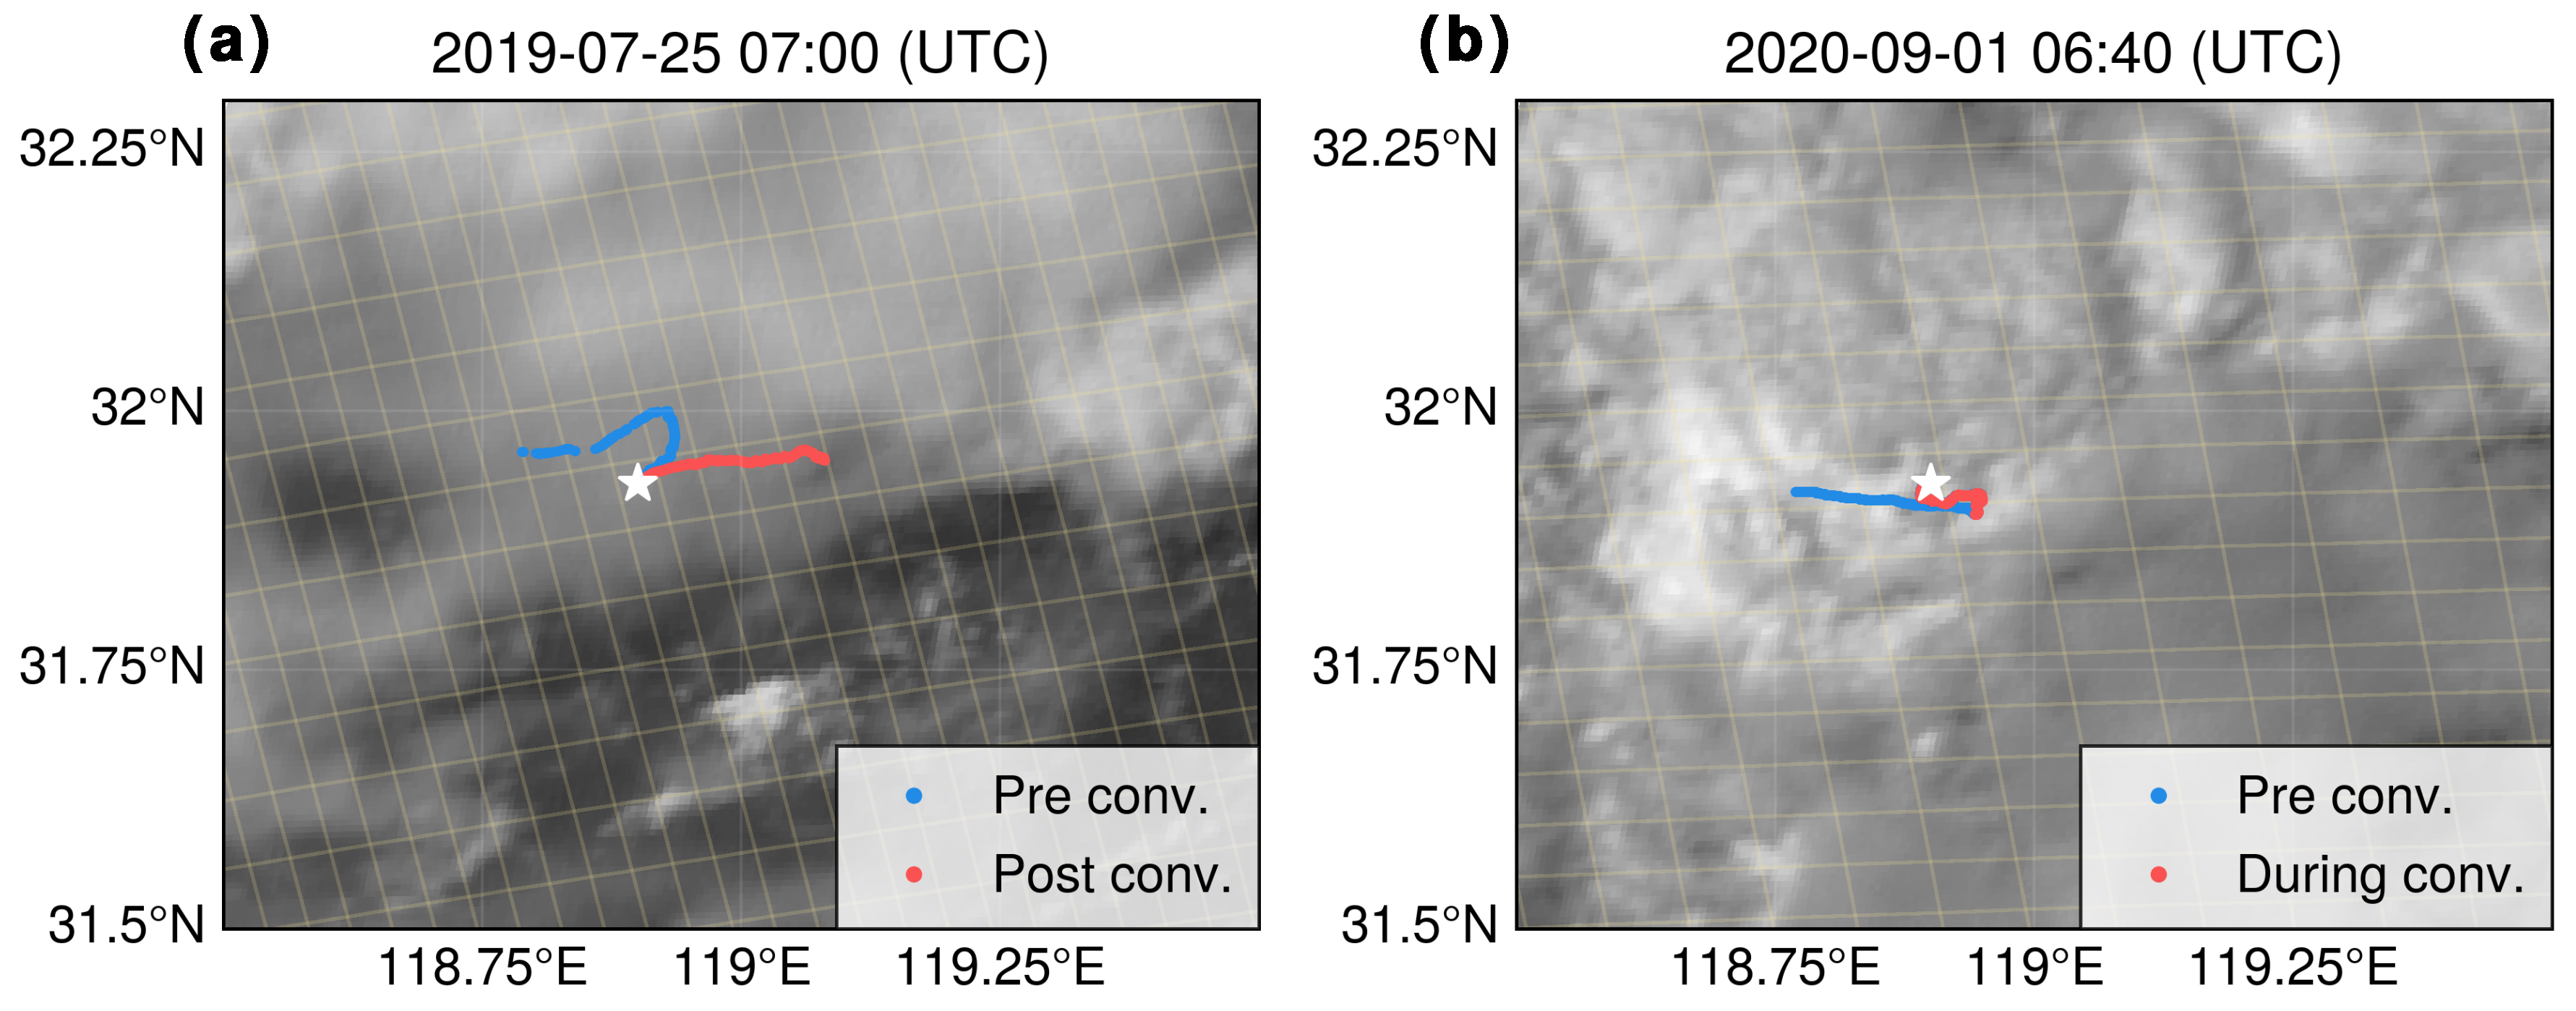
\includegraphics[width=35em]{./figures/ozonesonde.png}
\caption{(a, b) 在对流后/对流中的臭氧探空仪达到约 10 km时,风云4A先进地球静止辐射成像仪(AGRI)可见通道(0.65 $\mu$m)探测到的对流。
对流前的臭氧探空仪轨迹为为蓝色,其他为红色。白星符号代表观测站,细黄线是TROPOMI像素条带。
图(c)和(d)是在对流前(虚线)和对流后/对流期间(实线)探空观测到的O$_3$(红色)和Q$_v$(黑色)廓线。
模式初始(虚线)和对流后或对流期间(实线)的O$_3$廓线为蓝色。
深灰色阴影是50\%的置信区间,浅色是90\%的置信区间,灰线是第一对流层顶。}
\label{figure:ozonesonde}
\end{figure}


具体而言,2019年7月25日发生的对流为热对流,释放的三个臭氧探空均产自中国大气物理研究所(IAP)。
IAP 臭氧探空仪使用电化学浓差电池 (ECC),其完整参数和性能见\citet{Zhang.2014}。
总体而言,从地表到2.5 km平均偏差小于0.3 mPa,9 km以下接近零,9--18 km之间小于0.5 mPa。
释放的第一台IAP臭氧探空仪于7月23日(晴天)05:35 UTC释放,另外两台分别于7月25日05:10 UTC(对流前)和06:35 UTC(对流后)释放。
由于防水故障,对流前释放的探空仪在释放后几秒钟就失去了信号,故而我们选择了7月23日释放的臭氧探空仪作为对流前的数据。
虽然时间间隔为2天,但10 km以上预报的O$_3$剖面最大相对差异通常小于25\%(图\ref{figure:waccm_forcast_o3})。
因此,臭氧日变化不足以解释探空观测到的超过65\%的差异。

此外,两台维萨拉(VAISALA)ECC臭氧探空仪分别于8月31日23:45 UTC(对流前)和9月1日06:10 UTC(对流期间)成功释放。
准备工作及具体操作均遵循标准手册,确保精度优于5\%,且在30 km 以下的精度在$\pm$ (5--10) \% 以内\citep{Smit.2007}。
该次探空试验所捕获的飑线是由冷空气和台风梅萨克(Maysak)外围环流的汇合发展而来的。
值得强调的是,对流期间的臭氧探空仪直接穿入云层,为探索受对流云影响的臭氧提供了独特的机会。



\begin{figure}[htbp]
\centering
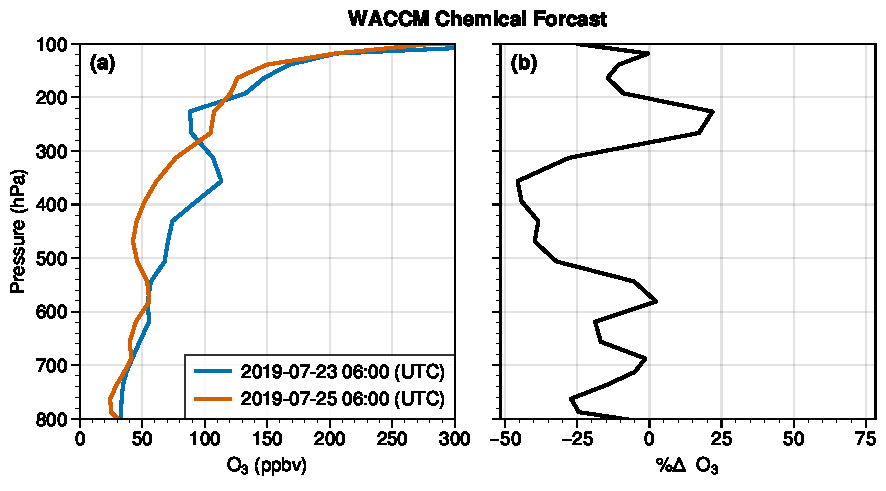
\includegraphics[width=35em]{./figures/waccm_forcast_o3.pdf}
\caption{(a)WACCM预测的区域平均(118.5$^{\circ}$E -- 119.5$^{\circ}$E, 31.5$^{\circ}$N – 32.5$^{\circ}$N)臭氧廓线。
蓝色为对流前,橙色为对流后。(b)为(a)中O$_3$剖面的百分比差异。}
\label{figure:waccm_forcast_o3}
\end{figure}

\subsection{闪电数据集}

在北极的研究中,我们使用了维萨拉全球雷电数据集(GLD360)。
该闪电探测网建立于2009年,由全球极低频闪电探测传感器组成,可检测地闪和云闪\citep{Said.2010,Said.2013,Said.2017}。
地闪和云闪在北极洋面上的探测效率分别为50\%--60\% 和 < 10\%\citep{Vagasky.2022}。
因此,我们使用恒定的云闪地闪比率(约 1)来计算总闪,即修正后的总闪电为检测到的地闪的四倍\citep{Mackerras.1994,Prentice.1977}。

在美国大陆的研究中,我们使用了整体闪电探测网(ENTLN; \citet{Marchand.2019})。
ENTLN运营着一个由全球1500多个地面站组成的系统,在美国大陆安装有900多个传感器\citep{Zhu.2017}。
云闪和地闪均由传感器根据电场脉冲极性和波形进行定位,检测频率范围为1 Hz 至 12 MHz。
如果脉冲组在700 ms和10 km范围内,则它们被归类为闪电。
在ENTLN的预处理数据中,包括了闪击和由一个或多个闪击组成的闪电。
\citet{Rudlosky.2015}将ENTLN组合事件(云闪和地闪)与闪电成像仪(LIS)测得的闪电进行了比较,
发现ENTLN在美国大陆上的闪电探测效率从2011年的62.4\%增加到2013年的79.7\%。
\citet{Lapierre.2020}还将 ENTLN 和 NLDN 数据集与2014年LIS的数据进行了比较,发现云闪闪电和闪击的探测效率分别为88\% 和 45\%。
由于我们和\citet{Lapierre.2020}一样仅使用2014年的ENTLN数据,我们采用同样的方法得到总闪的量。
具体而言,云闪闪电除以0.88,云闪闪击除以0.45,而地闪由于探测效率高,故不进行矫正。

在中国东南部的研究中,我们融合了三种闪电数据集:中国国家闪电探测网(CNLDN; \citet{Yang.2015})、
ENTLN和全球闪电定位网(WWLLN;\citet{Rodger.2006})。
江苏省CNLDN数据的地闪闪电探测效率约为90\% \citep{Li.2017a},
而ENTLN和WWLLN以特定的频率(ENTLN 为 1 Hz -- 12 MHz,WWLLN 为 3--30 kHz)同时探测云闪和地闪。
WWLLN的详细处理算法由\citet{Rodger.2004}给出。
在 10 km 和 0.7 s的条件下,WWLLN测得的闪击和脉冲与ENTLN融合,构成一个数据集(ENGLN,\citet{Virts.2020b})。
为了增加我们研究中的闪电数据覆盖范围,使用 10 km 和 0.5 s 的时空聚类标准将ENGLN和CNLDN数据集的地闪数据相结合\citep{Zhao.2020},合并后的数据集应具有足够高的地闪探测效率。
由于该三种闪电数据在中国范围内的云闪探测效率较低,我们保守地使用恒定的云闪与地闪比率(3:1,\citet{Wu.2016,Bandholnopparat.2020})来得到总闪数据。
若将来有更多的中国闪电网(如北京闪电网络(BLNET;\citet{Srivastava.2017})可用于与闪电成像传感器进行比较\citep{Rudlosky.2013,Poelman.2020},云闪数据将更加准确。

\section{卫星观测}

\subsection{臭氧监测仪(OMI)}

臭氧监测仪(OMI)搭载在Aura卫星(2004年发射)上,该卫星是下午列车(A-train)卫星组的成员\citep{Levelt.2006,Levelt.2018}。
OMI在$\sim$13:45 LT(升交点)经过赤道,条带宽度为2600 km,星下点分辨率为13 km $\times$ 24 km。
自2007年初以来,由于被称为“行异常”的异常辐射\citep{Dobber.2008},一些测量数据变得无效。
对于当前的研究,我们使用NASA标准产品v3.0\citep{Krotkov.2017}作为LNO$_x$反演算法的输入。

对流层NO$_2$垂直柱密度(V$_{\textrm{NO$_2$}}$)的计算主要包括以下步骤。

(1)NO$_2$总斜柱密度由 OMI 优化的差分光学吸收光谱(DOAS)拟合确定。

(2)通过从测量的总斜柱密度中减去由仪器引起的跨道偏差,得到校正(“去条纹”)的总斜柱密度。

(3)平流层(AMF$_{\textrm{strat}}$)或对流层(AMF$_{\textrm{trop}}$)的空气质量因子(AMF)是由考虑加权散射权重的NO$_2$先验廓线的垂直积分计算得到。
这些先验廓线是GMI模式模拟的月平均先验廓线(2004--2007 年)。

(4)平流层NO$_2$垂直柱密度(V$_{\textrm{strat}}$)是通过减去对流层NO$_2$的先验贡献和三步(插值、过滤和平滑)算法计算得出\citep{Bucsela.2013}。

(5)V$_{\textrm{strat}}$ 使用 AMF$_{\textrm{strat}}$ 转换为斜柱密度,并从测量的总斜柱密度中减去,从而得到对流层NO$_2$斜柱密度(S$_{\textrm{NO$_2$}}$),进而 V$_{\textrm{NO$_2$}}$ = S$_{\textrm{NO$_2$}}$/AMF$_{\textrm{trop}}$。

(6)基于这种方法,我们开发了一种新的 AMF$_\textrm{LNO$_x$}$,通过替换原来的步骤来获得所需的 V$_\textrm{LNO$_x$}$(V$_\textrm{LNO$_x$}$ = S$_{\textrm{NO$_2$}}$/AMF$_\textrm{LNO$_x$}$)。

(7)该算法的具体细节将在\ref{section:lnox}节中讨论.

\subsection{对流层观测仪(TROPOMI)}

2017年10月13日,搭载对流层观测仪(TROPOMI)的哨兵5号(Sentinel-5 Precursor)卫星成功发射\citep{Veefkind.2012}。
对于本文的研究,我们使用Sentinel-5P产品算法实验室(S5P-PAL)再处理产品(v2.3.1)。
与v1.2/v1.3版本相比,新版本的产品包含的尖峰去除功能,以更好地处理探测器饱和和光晕效应,从而在对流产生的明亮云层上提供更有效的数据\citep{Ludewig.2020,VanGeffen.2022}。
其中具有较大检索错误(processing\_quality\_flags > 0)的像素被过滤掉。

与OMI一样,AMF$_{\textrm{trop}}$取决于多个参数(太阳天顶角、观察天顶角、相对方位角、表面反照率、地表气压、云分数、云高度和先验廓线):

\begin{equation} \label{eq:AMF_NO2}
AMF_{\textrm{trop}} = \frac{(1-f_r) \int_{p_{surf}}^{p_{tp}} w_{clear}(p) NO_2(p) \: dp + f_r \int_{p_{cloud}}^{p_{tp}} w_{cloudy}(p) NO_2(p) \: dp}{\int_{p_{surf}}^{p_{tp}} NO_2(p) \: dp}
\end{equation}

简而言之,分子是模拟的S$_{\textrm{NO$_2$}}$,分母是模拟的V$_{\textrm{NO$_2$}}$。
其中p$_{surf}$是表面压力,p$_{tp}$是对流层顶气压,p$_{cloud}$是云压,f$_{r}$是NO$_2$窗区中的云辐射率分数,
w$_{clear}$和w$_{cloudy}$分别是查找表中的气压相关散射权重(分别用于晴天和多云条件,\citet{Lorente.2017}),
NO$_2$(p)是示踪剂模型v5(TM5)模拟的NO$_2$垂直廓线。

云压是由477 nm附近O$_2$-O$_2$碰撞吸收带反演得到的反射率加权气压\citep{Acarreta.2004,Sneep.2008,Stammes.2008}。
故深对流云的云压位于几何云顶下方,其中几何云顶与云探测卫星(CloudSat)和中分辨率成像光谱仪(MODIS)等热红外传感器检测到的值更接近\citep{Vasilkov.2008,Joiner.2012}。
因此,OMI或TROPOMI测量的对流层NO$_2$大部分位于云内部,而不是云顶之上。
下文中,“云上”或“云下”都是相对于OMI或TROPOMI测得的云压而言。
\citet{Beirle.2009}的敏感性研究比较了云底和云顶的化学成分,发现云中大部分来自闪电的二氧化氮可以被卫星探测到。
云压的概念不仅应用于LNO$_x$的研究,还应用于计算上对流层O$_3$和NO$_x$的云切片方法\citep{Ziemke.2009,Choi.2014,Strode.2017,Ziemke.2017,Marais.2018}。

\subsection{闪电氮氧化物的反演} \label{section:lnox}

基于AMF$_{\textrm{trop}}$,为了得到对流层LNO$_2$或LNO$_x$的垂直柱密度,我们只需将分母改成LNO$_2$或LNO$_x$的垂直积分即可。

\begin{equation} \label{eq:AMF_LNO2}
AMF_{\textrm{LNO$_2$}} = \frac{(1-f_r) \int_{p_{surf}}^{p_{tp}} w_{clear}(p) NO_2(p) \: dp + f_r \int_{p_{cloud}}^{p_{tp}} w_{cloudy}(p) NO_2(p) \: dp}{\int_{p_{surf}}^{p_{tp}} LNO_2(p) \: dp}
\end{equation}

当研究区域为清洁区域,式(\ref{eq:AMF_LNO2})的分子可用LNO$_2$代替NO$_2$,即

\begin{equation} \label{eq:AMF_LNO2}
AMF_{\textrm{LNO$_2$Clean}} = \frac{(1-f_r) \int_{p_{surf}}^{p_{tp}} w_{clear}(p) LNO_2(p) \: dp + f_r \int_{p_{cloud}}^{p_{tp}} w_{cloudy}(p) LNO_2(p) \: dp}{\int_{p_{surf}}^{p_{tp}} LNO_2(p) \: dp}
\end{equation}

为了与前人对比,我们定义了其他两种云上的AMF,

\begin{equation} \label{eq:AMF_NO2Vis}
AMF_{\textrm{NO$_2$Vis}} = \frac{(1-f_r) \int_{p_{surf}}^{p_{tp}} w_{clear}(p) NO_2(p) \: dp + f_r \int_{p_{cloud}}^{p_{tp}} w_{cloudy}(p) NO_2(p) \: dp}{(1-f_g) \int_{p_{surf}}^{p_{tp}} NO_2(p) \: dp + f_g \int_{p_{cloud}}^{p_{tp}} NO_2(p) \: dp}
\end{equation}

\begin{equation} \label{eq:AMF_LNO2Vis}
AMF_{\textrm{LNO$_2$Vis}} = \frac{(1-f_r) \int_{p_{surf}}^{p_{tp}} w_{clear}(p) NO_2(p) \: dp + f_r \int_{p_{cloud}}^{p_{tp}} w_{cloudy}(p) NO_2(p) \: dp}{(1-f_g) \int_{p_{surf}}^{p_{tp}} LNO_2(p) \: dp + f_g \int_{p_{cloud}}^{p_{tp}} LNO_2(p) \: dp}
\end{equation}

其中f$_g$为云几何分数。以上各式中的NO$_2$和LNO$_2$廓线均来自于WRF-Chem的模拟结果。
由于北极地区排放源及对流模拟结果不确定性较大,本文利用基于云压假设的高斯分布来代替廓线。
高斯分布的峰宽设置为60 hPa,峰位为最高(数值最低)的OMI/TROPOMI云压。
北极地区对流云的云压范围为130$\sim$987 hPa,主要集中于250--300 hPa最常见的值(图\ref{figure:pcld_ptropo})。
由于云内部的NO$_2$浓度高,而云层之上的NO$_2$由于光解作用而浓度低,故假设的LNO$_2$廓线更加现实\citep{Beirle.2009}。
对于高而厚的云层,云层上方的散射权重相当均匀,LNO$_2$的灵敏度在云层中部附近最高,所以受LNO$_2$廓线假设的影响已降到最低\citep{Laughner.2017}。

\begin{figure}[htbp]
\centering
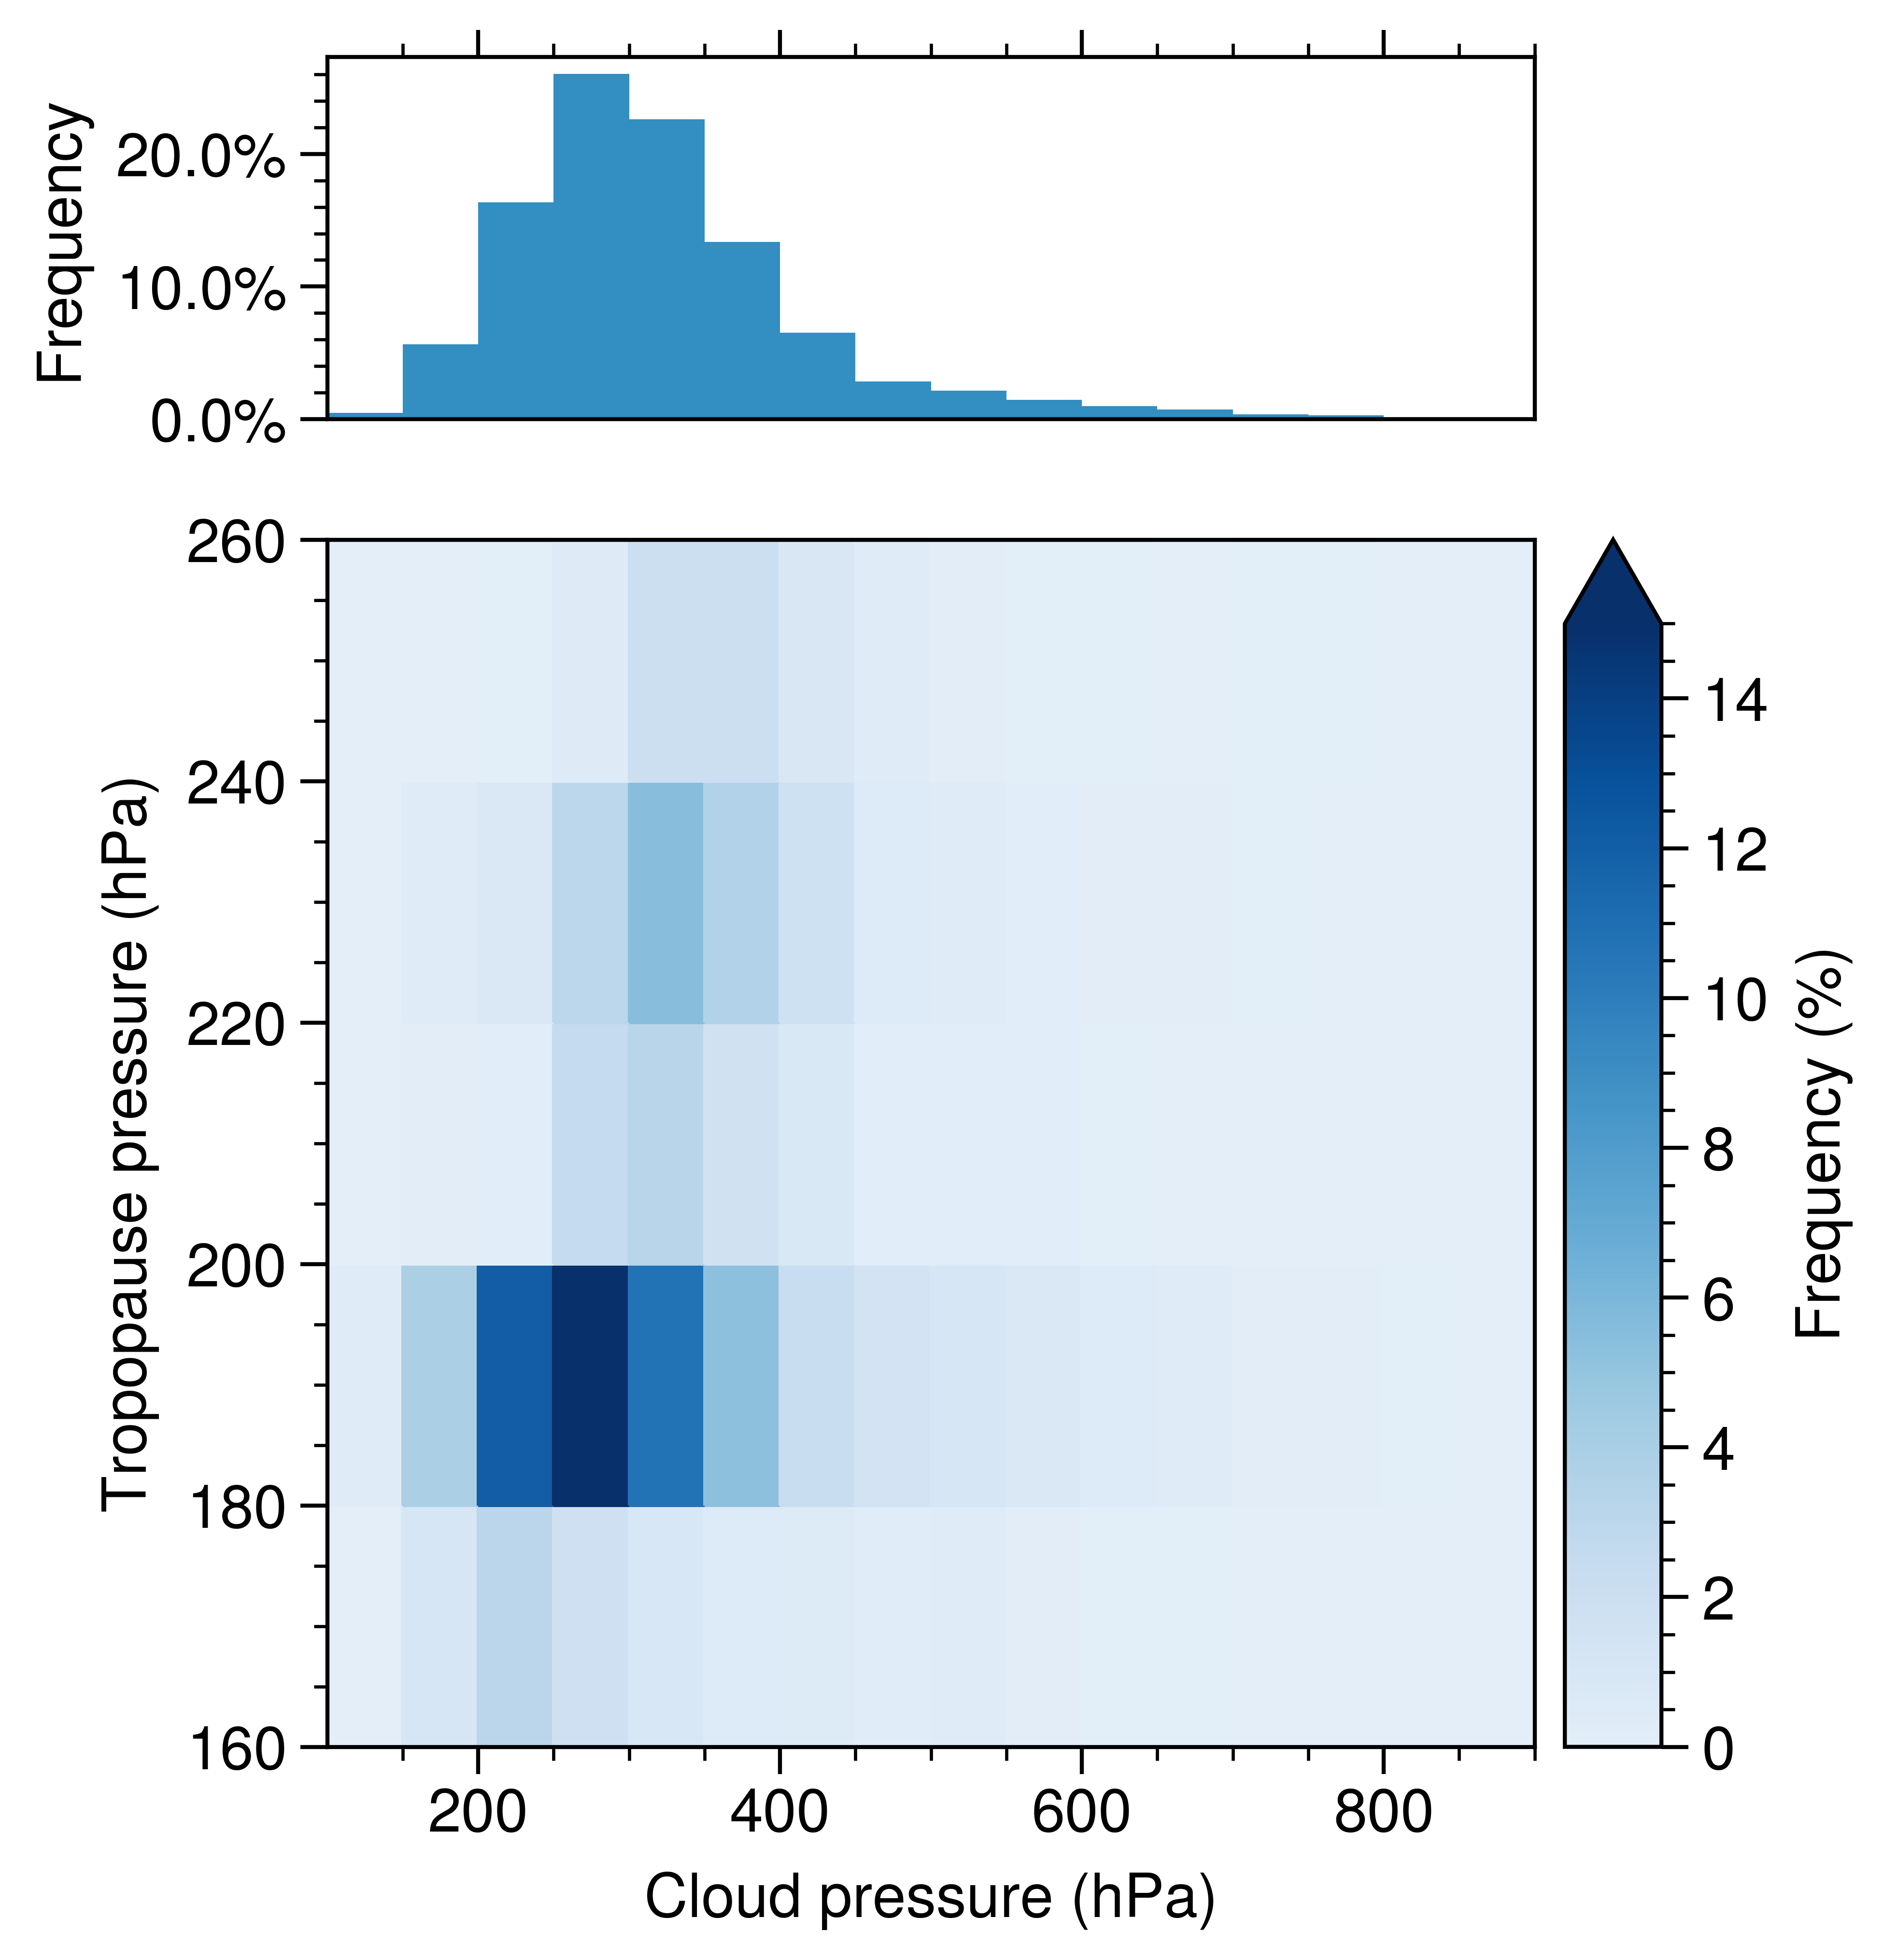
\includegraphics[width=20em]{./figures/pcld_ptropo.png}
\caption{云辐射分数大于0.7的像素上TROPOMI测得的云压和对流层顶高度直方图。}
\label{figure:pcld_ptropo}
\end{figure}

\section{模式设置}

\subsection{气象设置}

针对美国大陆地区的研究使用的WRF-Chem版本为3.5.1,水平网格大小为12 km $\times$ 12 km (图 ??a),垂直层数为29层,时间步长为72 s。
气象条件的初始场和边界场为时间分辨率3小时的北美区域再分析(NARR)数据集,每3小时应用一次边界条件和四维数据分析(FDDA)逼近,
其中温度、水汽和水平风以0.0003 s$^{-1}$ 的系数逼近\citep{Laughner.2017}。
微物理过程采用Lin方案\citep{Lin.1983},积云参数化为Grell 3D方案\citep{Grell.1993a,Grell.2002a},长波辐射采用RRTM方案\citep{Iacono.2008},短波辐射采用Goddard方案,陆面过程使用Noah陆面模式\citep{Koren.1999},边界层采用YSU方案\citep{Hong.2006}。
闪电参数化采用基于对流参数化的中性浮力水平\citep{Pickering.1992},云闪与地闪的比例基于\citet{Boccippio.2001}.

针对中国地区的研究使用WRF-Chem4.1.4,气象初始场和边界场来自1小时分辨率的欧洲中心大气再分析数据(ERA5,\citet{Hersbach.2020}),垂直层为75层,对流层顶为50 hPa。
嵌套设置如图??(b)所示。
微物理过程使用WSM6方案\citep{Hong.2006a},而短波和长波辐射使用RRTMG方案,陆面过程由Noah方案模拟。
但是,我们使用不同的边界层参数化来模拟两次对流个例,2019年的个例使用YSU方案,而2020年的隔离使用QNSE方案\citep{Sukoriansky.2005}。
闪电部分未使用参数化,用闪电同化代替,详见\ref{sect:lightning_assimilation}节。

\subsection{化学设置}

美国大陆地区研究采用臭氧和相关化学示踪剂模型第4版(MOZART-4;\citet{Emmons.2010})的输出场作为化学的初始场和边界场。
人为排放由2011年美国国家排放清单(NEI)驱动,并根据环境保护署年度总排放量,按模拟的年份进行调整\citep{EPA.2015}。
生物排放使用来自自然界的气体和气溶胶排放模型(MEGAN;\citet{Guenther.2006})。
化学机制是区域大气化学机制第2版(RACM2;\citet{Goliff.2013}),并由\citet{Browne.2014}和\citet{Schwantes.2015}进行了更新。
此外,LNO$_x$参数化采用每次闪电产生200 mol NO,调整因子为1,以下简称“1$\times$200 mol NO per flash”)。
基于\citet{Ott.2010}的双峰型闪电NO(LNO)廓线\citep{Laughner.2017}被用作 WRF-Chem中LNO的垂直分布,而LNO和LNO$_2$廓线是指有和没有闪电的模拟之间垂直廓线的差异。

中国地区研究采用整个大气社区气候模型(WACCM,\url{https://www.acom.ucar.edu/waccm/})的输出作为化学初始场和边界场。
其中2020年个例的初始O$_3$廓线使用臭氧探空仪观测所得的O$_3$廓线。
人为排放使用2016年中国多分辨率排放清单 (MEIC,\url{http://www.meicmodel.org/})1.3版驱动,生物排放采用MEGAN源。
化学机理使用气相化学的臭氧和相关化学示踪剂模式(MOZART)和气溶胶的Goddard化学气溶胶辐射和传输(GOCART)模式\citep{Pfister.2011}。
其中光解方案采用基于云光学厚度(cloud\_fraction$^{1.5}$)的新 TUV(对流层紫外线和可见光)方案,即光解速率依赖于气溶胶和云。
LNO的垂直廓线也采用双峰型\citep{Laughner.2017},而 LNO$_x$参数化调整为每次闪电产生500 mol NO\citep{Zhu.2019}。



\subsection{闪电资料同化} \label{sect:lightning_assimilation}

